\documentclass[12pt,letterpaper]{article}
\usepackage{graphicx}
\usepackage{wrapfig}
\usepackage{geometry}
\usepackage{fancyhdr}
\usepackage{xcolor}
\usepackage{lastpage}
\usepackage{vhistory}
\usepackage{hyperref}
% \usepackage{draftwatermark}
\usepackage{float}
\usepackage{array}
\usepackage{changebar}
\pagestyle{fancy}
\fancyhead{}

\lfoot{Beginning your flight training}
\cfoot{}
\rfoot{\thepage}
\renewcommand{\footrulewidth}{1pt}

\oddsidemargin=-10pt % Left margin; widened here with a negative value
\textwidth=7in % Text width
\setlength{\parindent}{0ex}

\begin{document}

\begin{center}

\begin{picture}(1000,1)
    \put(0,-50){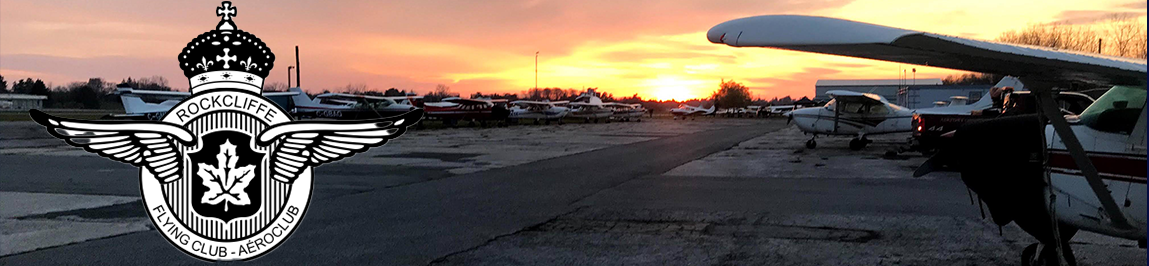
\includegraphics[width=\textwidth]{cyro-header.png}}
    \textcolor{white}{
    \put(190,16){\textbf{\small Guillaume Larose}}
    \put(190,4){}
    \put(190,-8){\small Flight Instructor}
    \put(190,-20){\small Rockcliffe Flying Club}
    \put(320,16){\small 1495 Sir George-Étienne Cartier Pkwy}
    \put(320,4){\small 613--746--4425 phone}
    \put(320,-8){\small 819--328--0825 cell}
    \put(320,-20){\small guillaume@rfc.ca}
    \put(320,-32){\small https://cyro.ca}}
\end{picture}

\end{center}
\vspace{16mm}

\centerline{ \large Beginning your flight training}

\tableofcontents
\setlength{\parskip}{1em}
    \section{Introduction}
    Beginning flight training may seem like drinking from a fire hose at first. This is a collection of resources and information that will be useful to understand more about your flight training. As you progress through the training, these subjects will be covered in more details but having a basic understanding will help make more sense of your training.

    \section{Resources}
    
        These are the official sources of information for aviation that you need to reference and get familiar with during your training. When available, this document will link to their online version.
    
        \subsection{AIM}
        The Transport Canada Aeronautical Information Manual (TC AIM) provides flight crews with a single source for information on rules and procedures for aircraft operation in Canadian airspace.
            
        This is a go to document for any question you may have on aviation procedures in Canada. You should get the latest copy online at \href{https://tc.canada.ca/en/aviation/publications/transport-canada-aeronautical-information-manual-tc-aim-tp-14371}{\color{cyan}{TP 14371}}.
        
        As you go through your ground school and training, read the corresponding chapters in the AIM. There are chapters on communications, aerodromes, rules of the air, VFR procedures around aerodromes, weather products, etc.

        \subsection{CFS}
        
        The CFS contains tables, legends and information to interpret the aerodrome directory which contains data and sketches of every Canadian aerodrome. It also contains general legends for other charts like VNC's and VTA's.

        \subsection{CARs}
        
        The CARs are the Canadian Aviation Regulations. They are the laws that govern aviation in Canada. The CARs came into force on October 10, 1996.
        
        Throughout this document, references to the CARs will be made by citing the article number in brackets like [602.96]. The CARs are available \href{https://tc.canada.ca/en/corporate-services/acts-regulations/list-regulations/canadian-aviation-regulations-sor-96-433}{\color{cyan}here}.
        
        \subsection{POH}
        
        Known as the Pilot Operating Handbook, this book is specific to the make, model and year of the aircraft. It contains information on the aircraft and how to operate it safely.
        
        The typical AFM/POH contains the following nine sections: General;
        Limitations; Emergency Procedures; Normal Procedures;
        Performance; Weight and Balance/Equipment List; Systems
        Description; Handling, Service, and Maintenance; and
        Supplements.
        
        You should go through the POH of the aircraft you will fly and get familiar with the different sections. Pay special attention to the general and systems sections as you will need to understand how the systems work in order to fly safely.
        
        \subsection{TP 6010}
        
        Canadian airspace is divided in several different classes and each class has specific rules that apply to it. At any given time in flight, we have to know which class of airspace we're in, whether it's controlled or not and who we should be talking to on the radio.
        
        TP 6010 is a publication by Transport Canada that gives you information on airspace classification and structure. The top part shows the rules for each classes and the bottom part displays visually how the different classes of airspace are arranged.
        
        You can google TP 6010 and print it as a reference.
        
        \subsection{Flight Test Guide}
        The flight test guide sets out the techniques, procedures and the marking criteria that will be used by Civil Aviation Inspectors and delegated Pilot Examiners for the conduct of the flight test required to demonstrate the skill requirements for the issuance of the Private Pilot Licence - Aeroplane. It is basically your contract with Transport Canada on how the exam will be conducted and what you will be marked on. You want to get familiar with this early in training. It is accessible \href{https://tc.canada.ca/en/aviation/publications/flight-test-guide-private-pilot-licence-aeroplane-tp-13723}{\color{cyan}here}.
        
    
    \section{Maps and airspace}
        \subsection{Airspace}
        All airspace in Canada is divided in different classes named A through G. Refer to TP 6010 to see the rules that apply to us in the VFR section. 
        
        You'll see that airspace is divided between controlled and uncontrolled airspace. Uncontrolled airspace is class G. Anything else is controlled airspace. They are named in order of how strictly controlled they are, A being the most strict and E being less strict.
        
        The airspace you're in can be determined from the maps -- we'll cover this in the next section. For example, around Ottawa we have a lot of class C airspace belonging to Ottawa Terminal that requires clearance to enter. A lot of the practice area is in class E which doesn't require clearance. Rockcliffe is in class G and is uncontrolled.
        
        \subsection{VNC}
        \begin{figure}
            \centering
            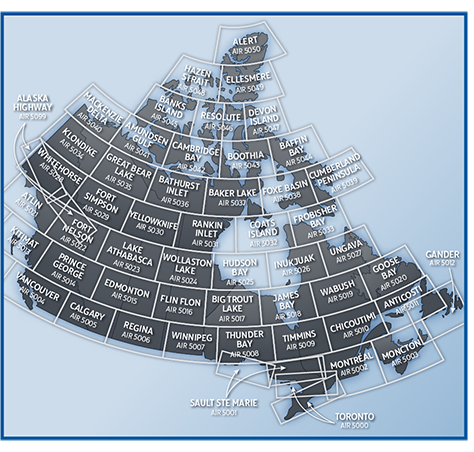
\includegraphics[scale=0.75]{vncs.png}
            \caption{VNC list}
            \label{fig:vnclist}
        \end{figure}

        The VFR Navigation Chart (VNC) is used by VFR pilots on cross-country flights at low to medium altitudes. The chart displays aeronautical information and sufficient topographic detail to facilitate air navigation. 

        Canada is divided in 52 such maps, as seen on Figure \ref{fig:vnclist}.
        
        \begin{figure}
            \centering
            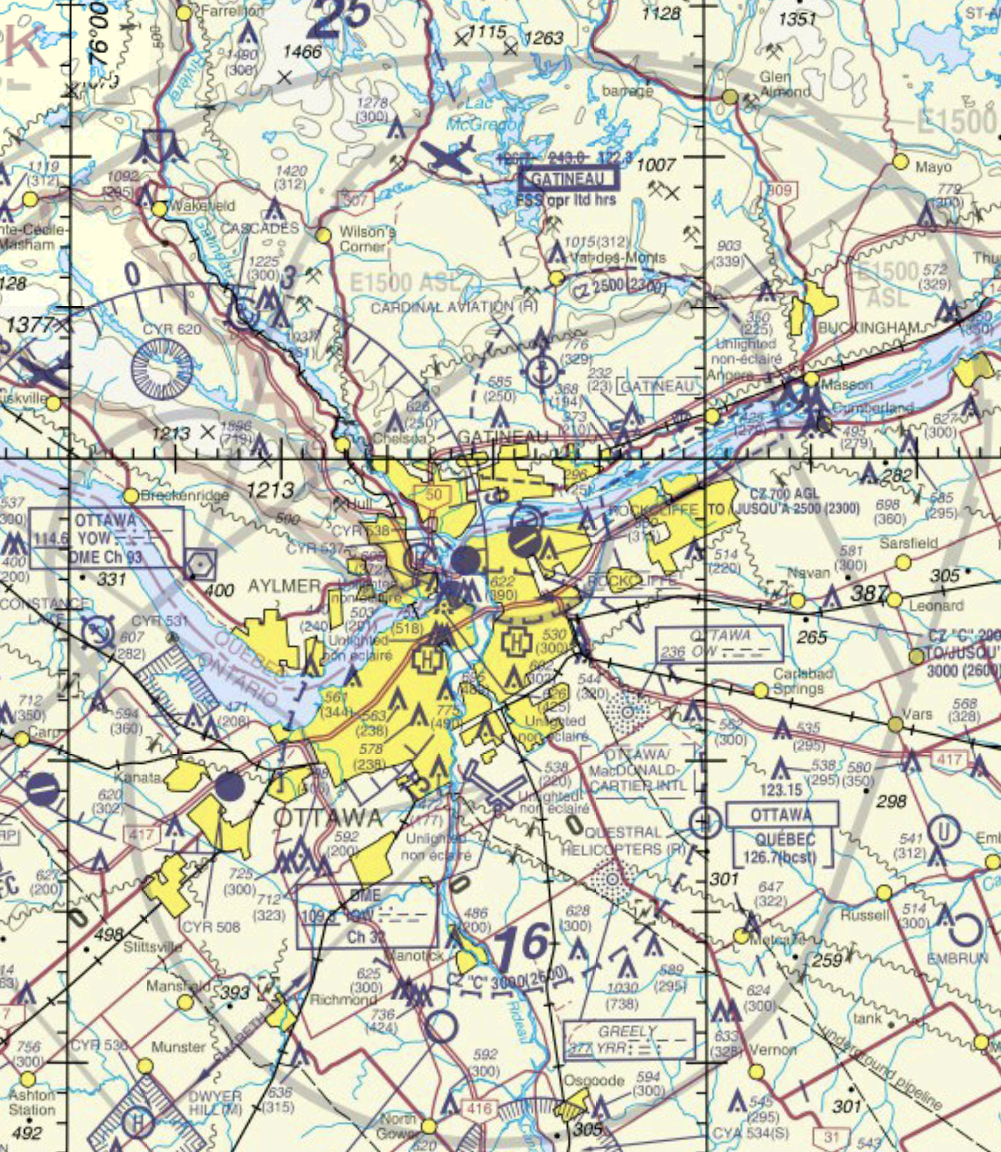
\includegraphics[width=0.75\textwidth]{vnc.jpeg}
            \caption{VNC}
            \label{fig:vnc}
        \end{figure}

        Ottawa falls in both the eastern edge of the Toronto VNC and the western edge of the Montreal one. Figure \ref{fig:vnc} is Ottawa on a VNC.
        
        \subsection{VTA}
        \begin{figure}[H]
            \centering
            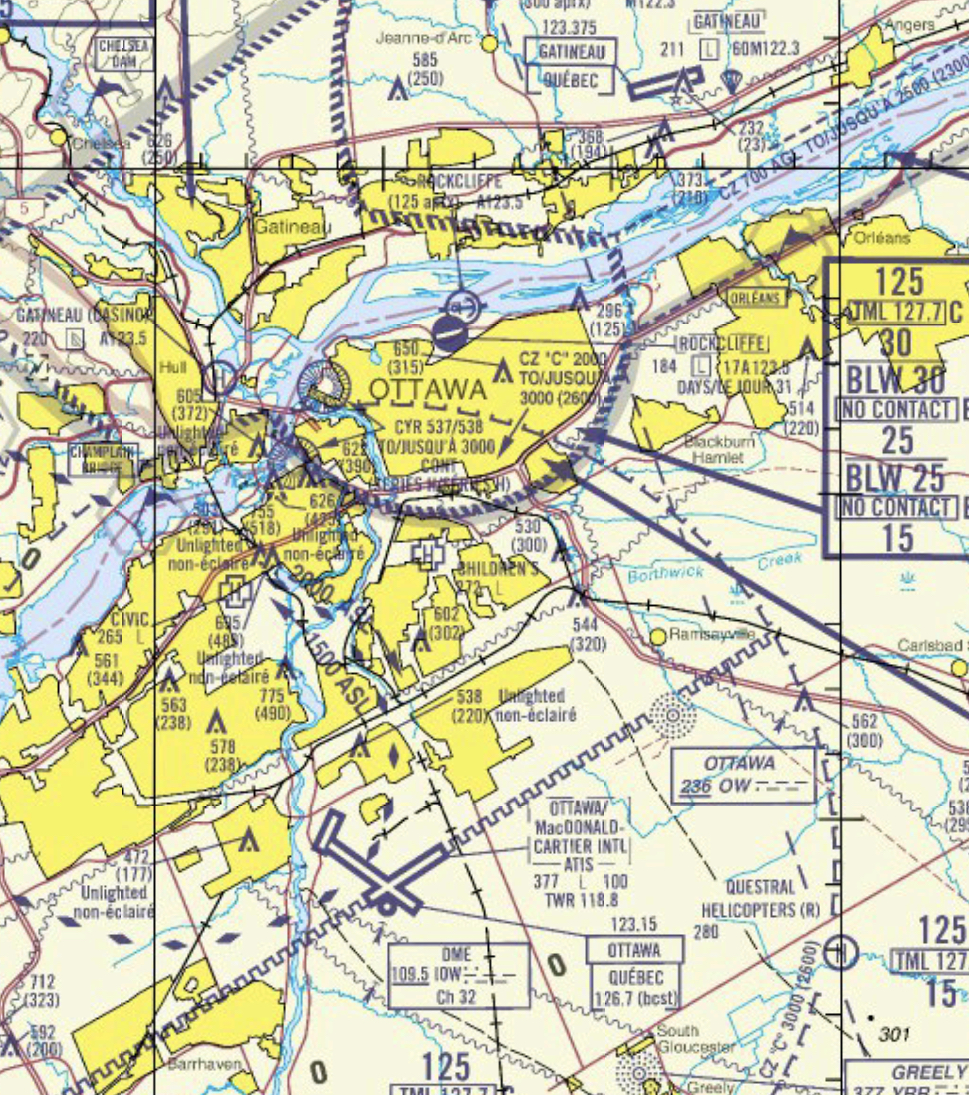
\includegraphics[width=0.75\textwidth]{vta.jpeg}
            \caption{VTA}
            \label{fig:vta}
        \end{figure}
        
        As you can see, the Ottawa area is quite busy and there are a lot of details in a small area of the map. For this reason, in congested traffic areas like Toronto, Ottawa or Vancouver, VTA charts are published. They provide a zoomed in view of the area and allow more details such as airspace to be shown on the chart.
        
        Figure \ref{fig:vta} is the same Ottawa area on the VTA. Rockcliffe airport is in the middle along the Ottawa river and is shows as a blue circle with a white line through it.
        
        One thing to note is that within the TCA (Terminal Control Area), airspace is clearly marked on the chart. Figure \ref{fig:airspace} shows how airspace is displayed. 
        
        \begin{figure}[h]
          \begin{center}
            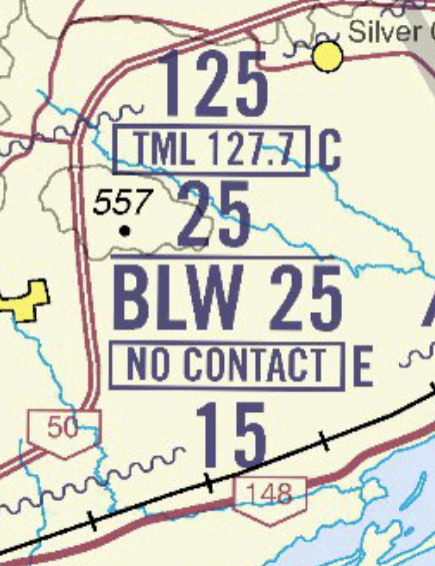
\includegraphics[scale=0.25]{airspace.jpeg}
          \end{center}
          \caption{Airspace}
          \label{fig:airspace}
        \end{figure}

        In this example, it shows class E airspace starting at '15' hundred feet (i.e. 1500'). That airspace extends to just below 2500'. At 2500' class C airspace starts and brings along a new set of rules. On top of it, it shows we should be talking to TML (Ottawa Terminal, an Air Traffic Controller) on frequency 127.7. Below 1500' is not noted therefore is uncontrolled, class G.
        
        Where there is no room for airspace to be detailed, it is displayed somewhere else on the map within a black box. That box has an arrow that points to where the airspace applies to.
        
        The airspace at Rockcliffe is in such a box that you can see on Figure \ref{fig:vta}.
        
        \subsection{Local area procedures and landmarks}
        \label{subsection:localprocs}
        
        The Rockcliffe Airport is a busy airport environment with constant training traffic and many visitors. It is an uncontrolled airport meaning there is nobody on the ground that keeps track or directs traffic. All aircrafts broadcast their position and intentions on the radio and it's up to the pilots to sort out conflicts. The following procedures have been developed to help provide separation between incoming and outgoing traffic.
        
        \begin{figure}
          \begin{center}
            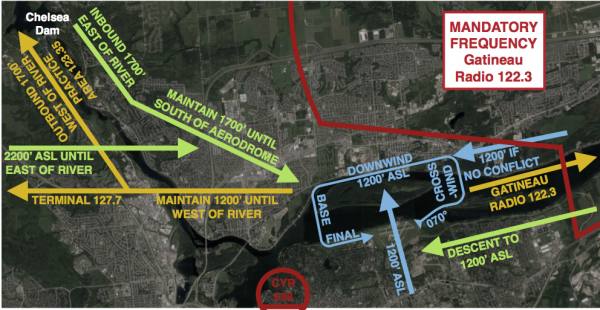
\includegraphics[width=0.6\textwidth]{cyro-local.png}
          \end{center}
          \caption{Local Procedures}
          \label{fig:local-procedures}
        \end{figure}

        Aircraft taking off and landing at Rockcliffe fly a rectangular pattern on the north side of the airport at 1200'. To keep 500' separation with the traffic coming back from the practice area, that traffic should stay at 1700', east of the Gatineau river, until south of the airport.
        
        This also means departing traffic should not climb above 1200' until west of the Gatineau river to stay out of the way of the incoming traffic. There is also traffic coming in from the west that will overfly all the previous traffic at 2200' until they talk to each other to sort out any conflicts. Figure \ref{fig:local-procedures} depicts these procedures.
        
        
    \section{Transponder, radar and ATC}
        \subsection{Primary and Secondary Radar}
        Air traffic controllers rely on radar to see the position of aircrafts, their identity, speed and altitude.
        
        Primary radar simply emits radio waves in all directions and big objects like aircrafts reflect that wave back at the sensor. This doesn't require any equipment inside the airplane and gives pretty accurate position and speed but lacks identity and altitude.
        
        Secondary radar relies on aircraft transponders to operate. The radar broadcasts interrogation signals and transponders reply with a 4 digit code and their current altitude. The code identifies which aircraft this is and what they set out to do. Before our flights, we'll call a phone number and tell them who we are, what we're doing and they will assign us a 4 digit code.
        
        \subsection{Transponder modes}
        Transponders have multiple modes of operation which we'll use in different phases of flight. On the ground, we'll keep them on \emph{STANDBY} which means it will not reply to interrogations. Before takeoff, we'll switch it to \emph{ALT} which means it will start reporting our code and altitude. That's called Mode C. If you simply switch it to \emph{ON}, it would report our code but not our altitude, that's Mode A.
        
        \subsection{Flight Information Centers and Area Control Centers}
        In order to get a transponder code before our flight, we need to talk to someone either at a FIC or ACC.
        
        \begin{figure}[h]
          \begin{center}
            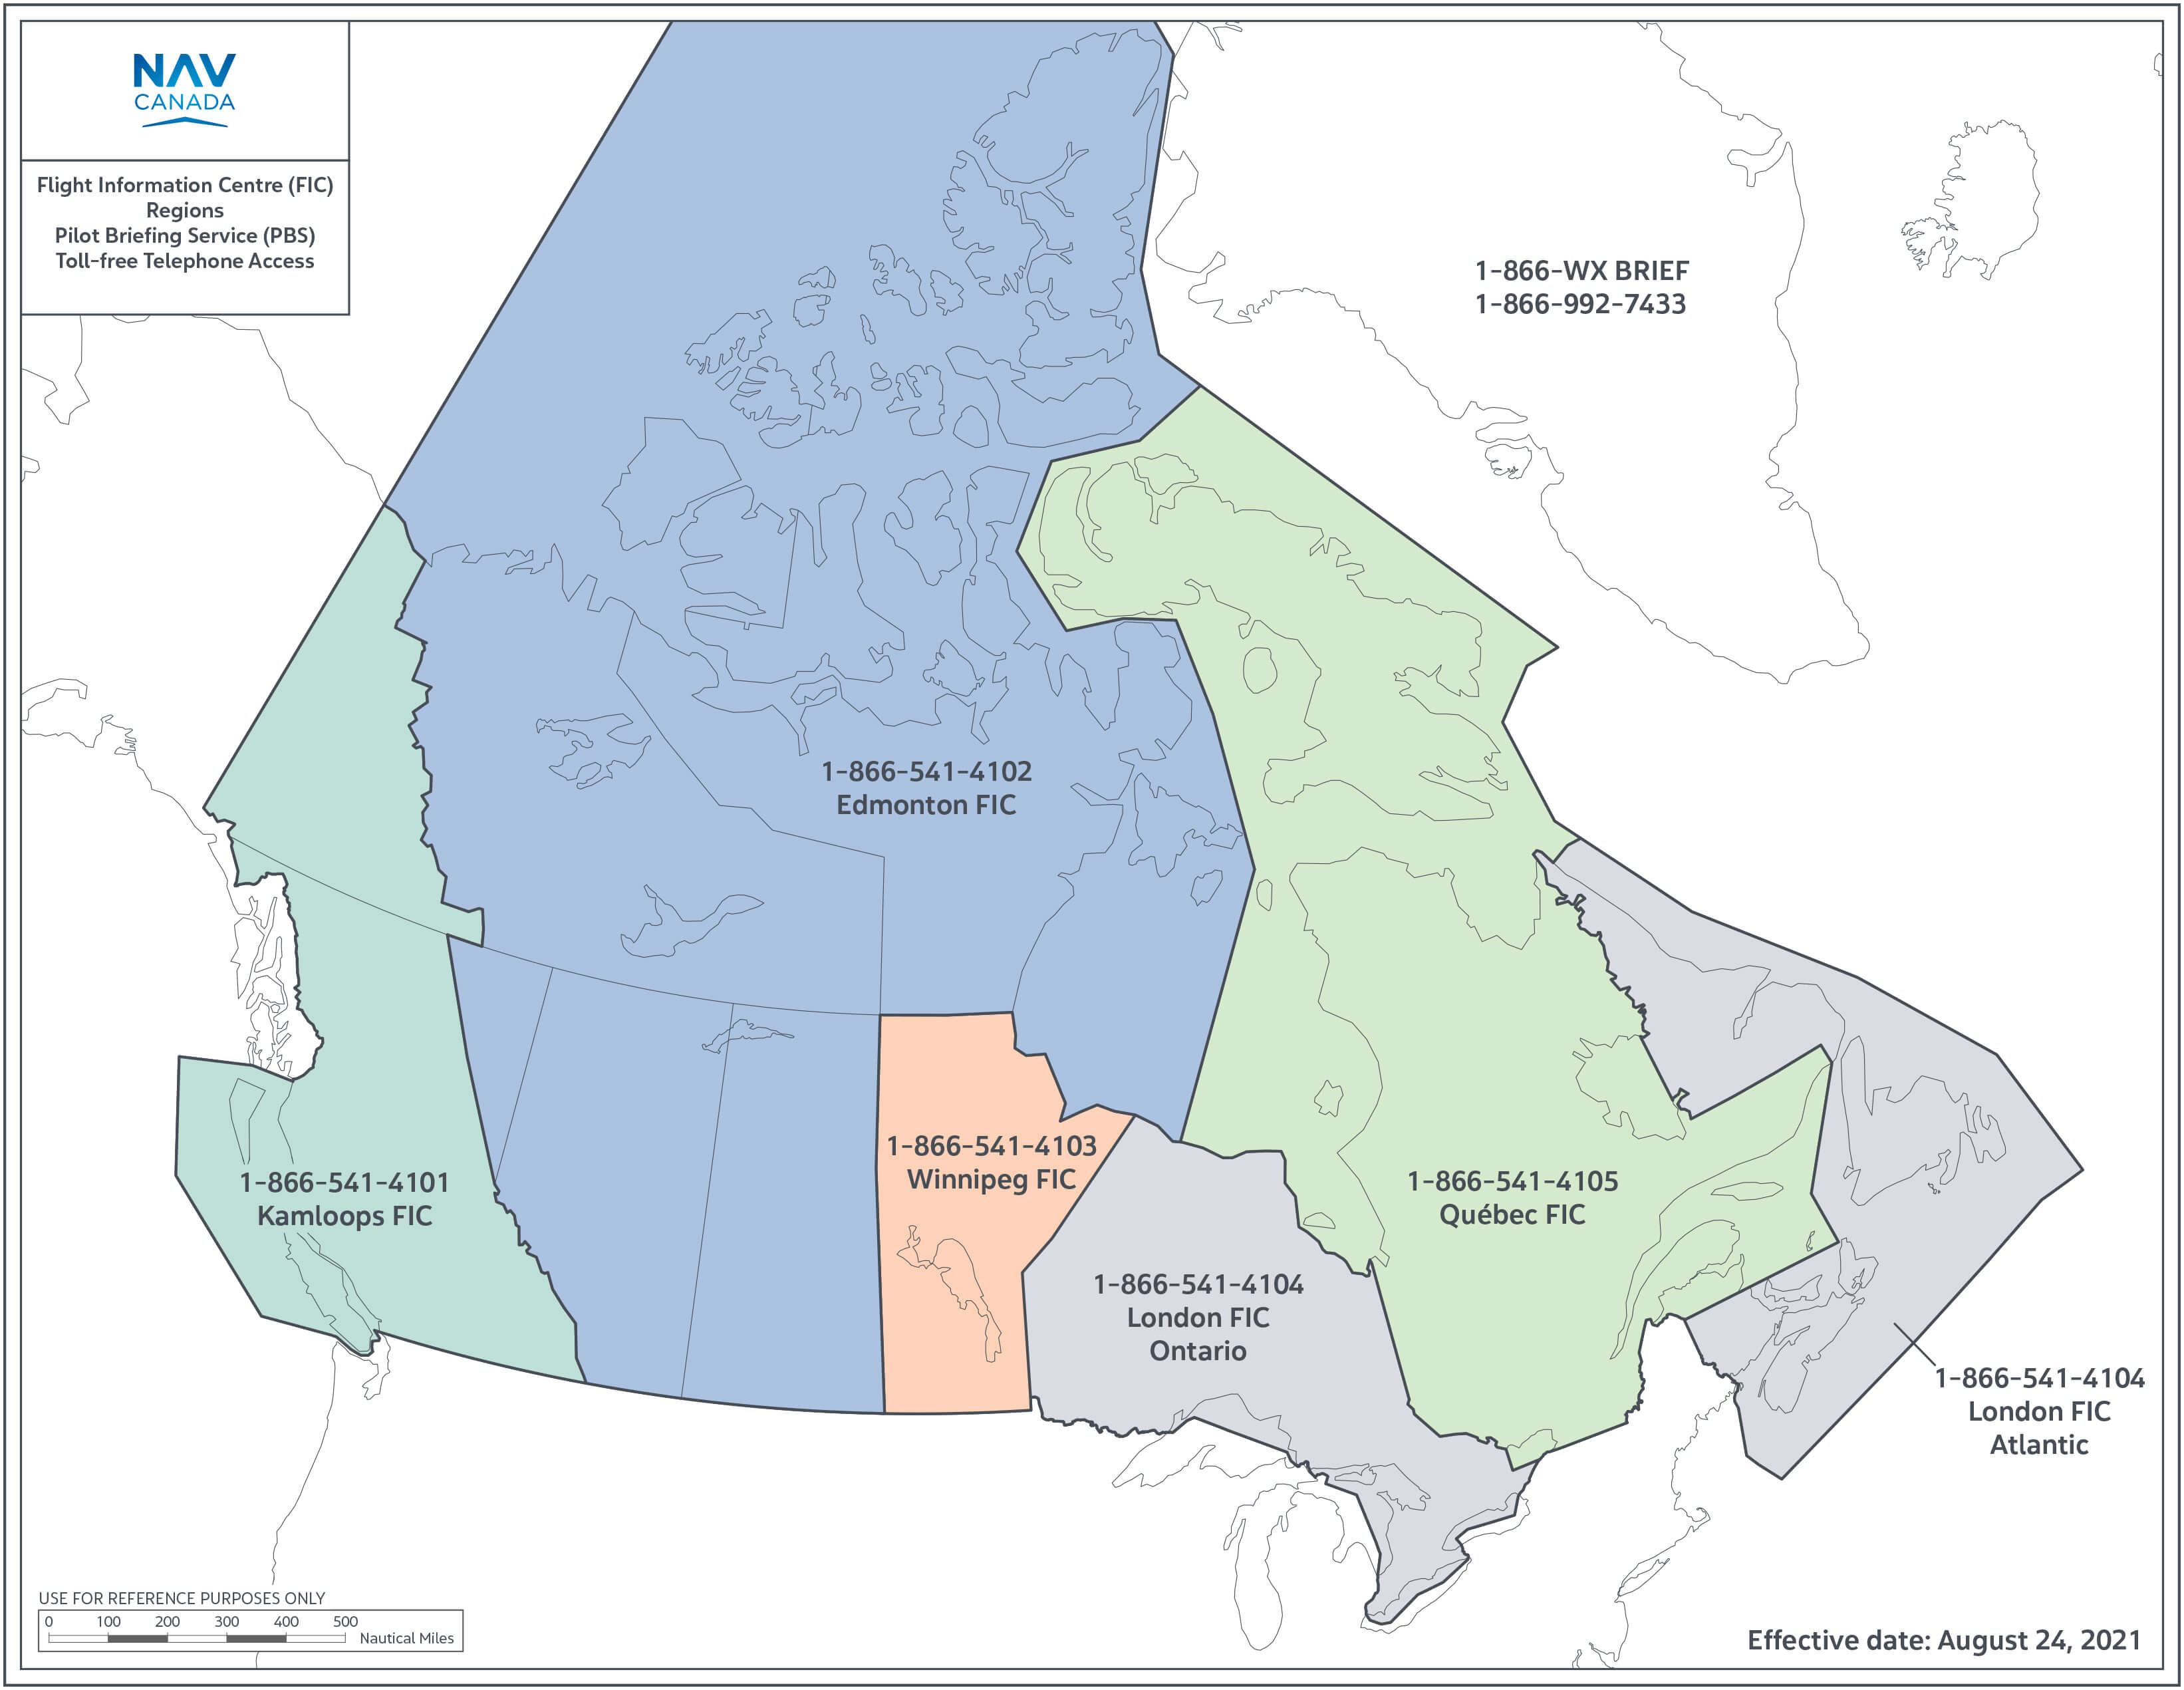
\includegraphics[width=0.6\textwidth]{fics.jpg}
          \end{center}
          \caption{FIC's}
          \label{fig:fics}
        \end{figure}

        Flight Information Centres (FIC's) are centres employing flight service specialists responsible for the management and dissemination of flight safety related information operated by Nav Canada. They can provide weather briefings, file flight plans or assign transponder codes. There are multiple FICs that cover different areas of the country. Figure \ref{fig:fics} shows the map.
        
        \begin{figure}[h]
          \begin{center}
            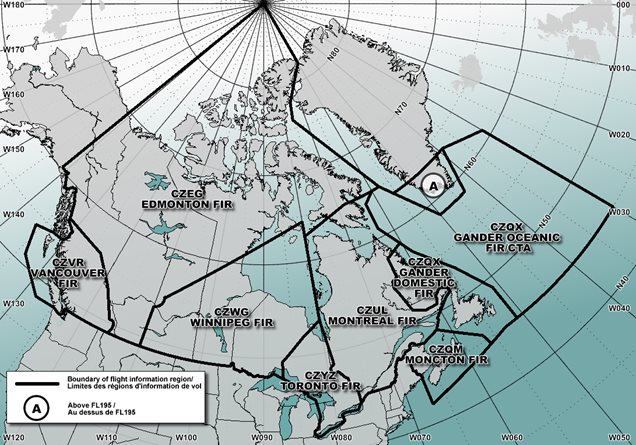
\includegraphics[width=0.6\textwidth]{firs.jpg}
          \end{center}
          \caption{FIR's}
          \label{fig:firs}
        \end{figure}

        Area Control Centers (ACC's), known simply as centers, are ATC facilities that control traffic flying through their flight information region (FIR). Again Canadian airspace is divided in multiple of these regions which you can see on Figure \ref{fig:firs}. These are not staffed by flight service specialists and will not provide flight planning help or weather briefings. This, however, means calling them for a simple transponder code is much faster and you don't have to wait in line.
        
        On the ground, you can reach Quebec FIC by calling 1-866-WX-BRIEF. WX stands for weather. You can reach Montreal Center by calling 1-866-VFR-CODE.

    \clearpage
    \section{Documents}
    \begin{samepage}
    
    Certain documents need to be carried on board during a flight and others need to be checked before the flight to ensure the required maintenance has been done on the aircraft. We use the JAILROW acronym to help remember them.
    
    \begin{itemize}
        \item \parbox[t]{0.4cm}{\textbf{J}} -- Journey Log
        \item \parbox[t]{0.4cm}{\textbf{A}} -- Certificate of Airworthiness (C of A)
        \item \parbox[t]{0.4cm}{\textbf{I}} -- Insurance
        \item \parbox[t]{0.4cm}{\textbf{L}} -- Licences and medical
        \item \parbox[t]{0.4cm}{\textbf{R}} -- Certificate of Registration 
        \item \parbox[t]{0.4cm}{\textbf{O}} -- Operating Handbook:  Pilot Operating Handbook (POH)
        \item \parbox[t]{0.4cm}{\textbf{W}} -- Weight and Balance
    \end{itemize}
    \end{samepage}

    \subsection{Journey Log [605.94] and [605.95]}
    
    The journey log must be carried on board unless the operator has a letter from the ministry that allows keeping it on the ground (e.g flight schools).
    
    As per [605.95], the journey log need not be carried on board for a flight if it is not planned to land and shut down the engine at another airport.
    
    Each flight and change of PIC must be entered on a separate line, unless:
    \begin{itemize}
        \item They are made by the same pilot, within 8 hours and within 25 NM of the departure point (e.g: glider towing, parachute drops)
        \item For a flying school, all flights are recorded and preserved on a daily flying sheet.
    \end{itemize}
    
    Defects must be entered in the Comments or Defects column unless the company maintenance manual provides for separate snag sheets.
    
    Entries must be in ink, and incorrect entry must be crossed out by a single line and initialed.
    
    Erasing, altering, or removing part of a logbook is a punishable offence.
    
    Journey logs must be kept for 1 years after the last entry date. [605.94]
    
    The last two entries of the old journey log are entered as the first two entries of the new log book.
    
    To verify that a journey log is up-to-date, and the aircraft is airworthy, check:
    \begin{itemize}
        \item Recent flights have been entered
        \item All airworthiness inspections have been completed and signed off by an AME
        \item Enough hours remain on the aircraft to complete the intended flight prior to the next inspection
        \item Snags or defects have been addressed and signed off by an AME
        \item Periodic inspections have been completed -- see subsection \ref{subsection:periodic}.
    \end{itemize}
    
    \subsection{Certificate of Airworthiness}

    The C of A is issued by Transport Canada to certify that the original design was airworthy.  Conventional aircraft (Cessna, Piper, etc) have a standard certificate of airworthiness. It is based on the original design, testing and manufacture approved by the FAA or TC. A special certificate of airworthiness can be issued for amateur-built aircraft, based on inspection by TC or a designated inspector during construction.  

    The C of A is issued when the aircraft is built, or when it is imported into the country. As per [605.03], it must be carried on board at any time the aircraft is flying. The C of A remains with the aircraft until it is exported or destroyed.

    For the C of A to remain valid and in force, the aircraft has to be deemed airworthy at the time of every flight.  This requires that:

    \begin{itemize}
        \item The aircraft must be in serviceable state, and all required equipment for flight are functioning [625.xx] including necessary instruments for the type of flight. [605.14] for day, [605.16] for night flights. Per [425.23] training aircrafts require a turn and bank or turn coordinator.
        \item Any airworthiness defect must be repaired, and the aircraft must be certified/signed off by an Aircraft Maintenance Engineer (AME). Defects which do not affect airworthiness (“Deferred Defects”) must be signed off as such by an AME and placards placed in the aircraft as required to advise flight crews. In a commercial operation, these deferred defects or un-serviceabilities will be indicated on an Aircraft Status board prominently displayed in the dispatch area.
        \item Airworthiness Directives (AD's or AWD's) must be complied with and the aircraft certified as airworthy by the AME. AWDs are notices issued by the aircraft/component manufacturers or FAA/TC to advise of required maintenance actions required due to recurring or recently discovered defects. AWDs can be one-time or recurring at different intervals (based on number of flight hours or calendar days). AWDs are relayed to aircraft owners through Transport Canada. A list of AWDs applicable to an aircraft can be found on Transport Canada’s web site. At Rockcliffe, we rely on the maintenance tracking system to ensure all AWDs are complied with. 
        \item Periodic inspections are completed as required. This is covered in the next section.
        \item The weight and center of gravity must be within limits. Aircraft must be operated under the category shown on the C of A and as confirmed by the weight and balance calculation.
        \item The required emergency equipment must be on board. 
        \item The baggage and any other objects must be secured.
        \item Unrestricted access must be available to all emergency exits.
    \end{itemize}

    If a C of A is rendered invalid then the insurance for the aircraft may not be valid. Therefore, if the aircraft is not being flown in accordance with the CARs and the POH, you may not be insured.

    The AAIR (Annual Airworthiness Information Report) is a report produced for Transport Canada updating registration and hours flown information. It is required to be filed every year prior to the due date. It is not a legal requirement that it be carried on board, but it is a common operations practice to include it with aircraft documents. If the AAIR is not completed or submitted, the validity of the C of A is not affected, but the owner will be liable for a fine.

    A Special C of A can be issued when an aircraft is fit for flight, but does not meet all of the requirements for a C of A.  An aircraft operating on a Special C of A can only be flown in Canadian Airspace. There are several different types:
    \begin{itemize}
        \item Provisional
        \item Restricted
        \item Amateur Build
        \item Limited
    \end{itemize}

    A Flight Permit is issued when an aircraft is capable of safe flight but does not meet the C of A or Special C of A requirements.  A Flight Permit is issued under two categories: experimental and ferry.
    
    Specific purposes for the issue of a flight permit are:
    \begin{itemize}
        \item Ferry flights to a base for repair or maintenance
        \item Importation or Exportation of an aircraft
        \item Demonstrations, Market Survey, Crew Training
        \item Testing following a repair, modification or maintenance.
    \end{itemize}
    
    When operating on a flight permit ensure all restrictions listed on the permit are checked prior to flying the aircraft.

    \subsubsection{Periodic Inspections}
    \label{subsection:periodic}
    
    Some required inspections are based on air time, others are on a fixed calendar schedule.
    
    An annual inspection is required for all aircraft that are not on Progressive Care, in particular private aircraft. The annual inspection can take multiple days to do, so commercial organizations use Progressive Care which breaks the inspection down into modules which are done at 50 hour intervals. Rockcliffe has its own program approved by Transport Canada.

    We rotate through 4 inspections, one every 50 hours of \emph{air time}. Each one covers different elements of the aircraft and includes a change of engine oil and filter, various other items, AWDs and fixing outstanding deferred defects.
    
    One 10 hour extension to the 50 hours may be granted by an AME before the 50 hours are used up as long as there are no AWDs due. After getting an extension, the next inspection cycle will be due in 40 hours instead so everything is back on schedule at 100 hours. An AME must sign off all inspections for the aircraft to be considered airworthy.

    The compass must be swung (calibrated) every 12 months and compass correction chart must be displayed in journey log and in the aircraft.

    The emergency locator transmitter (ELT) must be checked every year and batteries replaced every 5 years or per manufacturer recommendation. The airplane may be operated without the ELT for a period of 30 days if a placard is placed showing when it was removed. A training aircraft may operate without a placard if the flight is to be within 25nm of the airport of departure or engaged in a flight test. See sections [605.38] and [605.39].

    The Altimeter must be calibrated every two years if the aircraft is to be flown IFR. The Pitot Static System must also be calibrated and transponder correlation checked every two years for flight in Mode C airspace. This means the transponder’s encoding altimeter is checked against the airplane’s altimeter to ensure that they are producing the same reading. At the same time, the airspeed indicator is also checked.
    
    All aircraft must have a first aid kit and portable fire extinguisher on board as per [602.59]. These are considered safety items. [602.59] and [625 Appendix C] mention that fire extinguishers should be inspected regularly as per Canadian Standards Association or manufacturer's recommendation. The standard is to inspect portable fire extinguishers annually.
    
    Air operators are required to have specific contents in their first aid kit and it shall be inspected annually as per [705.90]. It is a strong recommendation for everyone else, such as an FTU, but not a requirement. It can be argued that the first aid kit, being a safety item, is covered under the general rule for safety items and as such it shall be inspected annually.

    \subsection{Insurance}
    
    All aircraft must carry Liability Insurance, the amount of which is determined by the number of passengers the aircraft is capable of carrying and the weight of the aircraft [606.02]. If the aircraft is not engaged in a commercial operation, a minimum of \$100,000 liability insurance is required for an aircraft with maximum takeoff weight of 2300 lbs, \$500,000 for an aircraft between 2300 and 5000 lbs. Regulations require a minimum liability insurance of \$300,000 times the number of passengers on board for an aircraft in commercial operation of weight less than 5000 lbs, excluding parachute drops.
    
    Private and Commercial registered aircraft must carry proof of insurance on board.
    
    Failure to fly the aircraft in accordance with the certificate of airworthiness and for commercial purpose when the aircraft is registered for private purpose may invalidate any insurance coverage.
        
    \subsection{Licences and medical}
    
    They must be valid, signed, appropriate for the weather and time of day and carried on board as per [401.03].
    \begin{itemize}
        \item student pilot or pilot’s licence
        \item medical certificate
        \item restricted radio certificate -- technically, it doesn't have to be on board. According to s38 of Part V of the Radiocommunication Regulations (SOR 96-484), the pilot must be able to produce the document within 48 hours of receiving a request by an inspector.
    \end{itemize}

    \subsection{Certificate of registration [202.26]}

    It is the official registration of the airplane with the Government of Canada. It lists the aircraft call sign, serial number, year of manufacture, owner’s name and address, and purpose (commercial, private).

    It is valid for the life of the aircraft, unless:
    \begin{itemize}
        \item There is a change of owner (sale of aircraft). The seller completes the postcard section of the Certificate of Registration indicating the reason for change (change of ownership or address), and mails it to Transport Canada within 7 days.
        
        The certificate of registration is completed by the buyer (both copies). The white page is sent as an application for the New C of R. The pink is kept with the aircraft until the new certificate of registration arrives. It is valid for three months after transfer of custody of the airplane or until the aircraft is resold or the permanent certificate of registration is received. Only the bill of sale is proof of ownership.
        
        \item The aircraft is on a lease with a specific end date. In this case, even if the lease is renewed, the original C of R expires at the given date and it has to be renewed as well.
        
        \item There is a change of address. You have to notify the minister within 7 days via the postcard section. The change of address stub is attached to the certificate of registration.

        \item There is a change of purpose: change from private to commercial or vice-versa.
        
        \item There is a change of nationality. An aircraft cannot be registered in Canada if it is registered in another country. You cannot fly an aircraft registered in a country other than the pilot licence you hold; for example, with a Canadian licence, you cannot fly a US registered aircraft. 
        
        \item Destruction of the aircraft. You must notify the director general – civil aeronautics.

        \item The certificate of registration is destroyed or rendered illegible: A fee must be paid for the re-issue.
    \end{itemize}

    \subsection{Operating manual (Pilot Operating Handbook)}
    
    The POH must be carried on board [605.04]; it must be for the exact model and year of manufacture. It lists operating limitations, performance, emergency and standard procedures and servicing specifications. The aircraft must be operated in accordance with the POH to keep the Certificate of Airworthiness valid. 
    
    \subsection{Weight and Balance [605.92]}
    
    The \emph{Weight and Balance Report} lists all the components of the aircraft, their weights, and positions and the overall empty weight, empty center of gravity, empty moment and disposable load. Be careful, aircraft built after 1975 use a standard basic empty weight which includes all fluids and unusable fuel. Older aircraft used empty weight or licenced empty weight which does not always include oil or unusable fuel. Refer to the specific POH weight and balance section for details.
    
    Specific W\&B should be calculated before each flight with knowledge of passengers, cargo and fuel.
    
    W\&B information is valid at the time of aircraft manufacture.  It must be updated at each modification/addition/removal of equipment that will affect its weight or position.  An amendment is issued showing what has been changed and revised empty weight \& moment. Any previous reports or amendments should be shown as “Superseded”.
    
    The aircraft must be weighted and the W\&B is recalculated when an AME or AMO judges that there have been too many small changes done by arithmetic only for the weight and balance report to be accurate.
    
    The latest amendment information must be used for the calculation of weight and balance prior to a flight, NOT what is in the examples provided in the POH.

    \subsection{Technical Logs}
    
    Technical logs are issued for each aircraft and record any inspections and/or maintenance to various parts of the aircraft. The Technical logs comprise:
    \begin{itemize}
        \item Airframe log
        \item Engine log (for each engine)
        \item Propeller log (for each propeller)
        \item Installation and modification log
    \end{itemize}
    
    Technical logs are not normally to be carried on board, stored or travel with the Journey Log.  This is to ensure that at least one copy of the maintenance record exists should the airplane be destroyed en-route. They are subject to the same rules as the Journey Log: timeliness, correction and accuracy.

    \subsection{Not to be carried on board}
    
    Personal log books and Pilot Training Record should not be carried on board. Your logbook may be carried on board if required to certify flights, for instance if you need to get your logbook stamped during a training cross-country.
    
    Technical log books are not normally carried on board, unless the airplane is being ferried for an inspection or for a transfer of ownership. These are issued for each aircraft and they record inspections and maintenance work.  
    
    Airframe logs, engine Logs, propeller logs and installation and modification logs should not be carried on board.
    
    \section{Radio calls}
    During your training flights you will have to communicate your position and intentions to other aircraft or air traffic controllers. Refer to the VFR Phraseology guide by Nav Canada to learn the basics such as the radio alphabet, how to pronounce numbers, etc. It is a very good guide to understand the radio communications between aircraft and ATC. It can be found \href{https://www.navcanada.ca/en/vfr-phraseology.pdf}{\color{cyan}here}.
    
    At Rockcliffe, a lot of our time is spent at the airport and in the practice area, where we simply broadcast our intentions to others on the radio. Every radio call is made in the same order: Who you’re talking to, who you are, where you are and what you want. Table \ref{tab:radiocalls} shows examples of the calls you’ll be making in a training flight.

    \begin{table}[]
    \hspace*{-1cm}
        \begin{tabular}{| p{0.30\linewidth} |  p{0.20\linewidth} | p{0.07\linewidth} |  p{0.40\linewidth} |}
        \hline
         When & Who you're talking to & Id & Position/Intentions\\
        \hline
     
        Radio check after start & Rockcliffe dispatch & GQUO & Radio check seat 1\\
        \hline
        
        On taxiway A waiting for traffic to land & Rockcliffe traffic & GQUO & Holding short runway 27\\
        \hline
        
        Prior to entering the runway & Rockcliffe traffic & GQUO & Immediate takeoff rwy 27\\
        \hline
        
        Prior to entering runway 09 to backtrack & Rockcliffe traffic & GQUO & Backtracking rwy 09 OR lining up rwy 09 with backtrack\\
        \hline

        Intentions after take-off, can be a call in itself or appended to your take-off call & Rockcliffe traffic & GQUO & Departing to the west, climbing to 1700’ for Chelsea dam\\
        \hline
        
        Arrival in practice area & Practice area traffic & GQUO & 1 mile south of Chelsea dam, 1700’, looking to work Cantley to Wilson’s corner\\
        \hline
        
        On way back after switching to Rockcliffe & Rockcliffe traffic & GQUO & 1 mile north of Chelsea dam, 1700’, inbound for the overhead procedure\\
        \hline
        
        If you’d like a field advisory (traffic, wind,..) & Rockcliffe UNICOM & GQUO & Requesting a fied advisory\\
        \hline
        
        Overhead from the north (dam) & Rockcliffe traffic & GQUO & Overhead the field, 1700’, southbound. Descending to join mid-right downwind rwy 27\\
        \hline
        
        Overhead from the south (after turn+descent) & Rockcliffe traffic & GQUO & Overhead the field, 1200’, to join mid-right downwind rwy 27\\
        \hline
        
        Turning final & Rockcliffe traffic & GQUO & Turning final, rwy 27, full stop\\
        \hline
        
        Clear of runway, exiting on taxiway Charlie & Rockcliffe traffic & GQUO & Clear of rwy 27 on Charlie\\
        \hline
        
        \end{tabular}
        \hspace*{-1cm}
        \caption{Common radio calls}
        \label{tab:radiocalls}
    \end{table}
    
    \subsection{Common wording}
    Here are common phrases you'll hear on the radio and what they mean:
    \begin{itemize}
        \item Lining up runway 27 (or taking position): You're going to taxi on the runway and 'line up' with the centerline and wait. Usually done when you will wait for another aircraft to taxi off the runway for example.
        \item Immediate take-off (or departure) runway 27: You will taxi onto the runway and takeoff without stopping or waiting. 
        \item The overhead procedure: The procedure depicted in subsection \ref{subsection:localprocs} where you fly over the circuit at 1700' to turn around and join the circuit at 1200'.
        \item Established Cantley to Wilson's Corner: We commonly pick 2 landmarks around which we're working. To keep everyone safely separated, we communicate to others where we are working.
    \end{itemize}

    \newpage
    \section{How to get to first solo}
    
    There are a few exams to pass and things to do in order to get to your first solo. You want to start to work on them early in your training so they don't become a roadblock closer to your solo. Here are the major ones.
    
    \subsection{Medical Certificate}
    You need to have a valid medical certificate to fly. If you haven't already, ask dispatch for a current list of CAME's (Civil Aviation Medical Examiner) and go get your medical done.
        
    \subsection{PSTAR}
    It used to be the \textbf{P}re-\textbf{S}olo \textbf{T}est of \textbf{A}ir \textbf{R}egulations. It was too easy so they renamed it to the Student Pilot Permit or Private Pilot Licence for Foreign and Military Applicants, Aviation Regulations. It is a closed book exam of 50 questions from a public question bank you have access to. You can google for a website called Robyn's PSTAR or search your phone's app store for PSTAR app to study. The website has a commentary section on the right that explains why each answer is right or wrong. The exam is done at the club and booked through dispatch.
        
    \subsection{Radio License}
    You need a license to legally talk on the radio while flying. It's called the ROC-A for Radio Operator Certificate -- Aeronautical. Reading the previous material for the PSTAR and the VFR Phraseology guide should be enough to pass this exam. The exam is done at the club and booked through dispatch.

    \subsection{Student Pilot Permit}
    Known as the SPP, this is the Transport Canada permit that lets you fly solo under instructor supervision. After you have passed the PSTAR and ROC-A, you can submit your application through one of our Authorized Person. They will need to see and take a copy of a proof of name, age and citizenship (e.g. passport).
    
    \subsection{In-flight exercises}
    Specific exercises need to be completed and signed out in your PTR as completed before you go solo. You'll see the list at the front of your PTR but they include things you will learn soon like stalls, spins and crosswind landings.

\newpage
\begin{versionhistory}
  \vhEntry{1.1}{2021--10--05}{GL}{Added Flight Test Guide, radio calls, JAILROW and pre-solo information}
  \vhEntry{1.0}{2021--09--22}{GL}{Created}
\end{versionhistory}

\end{document}